\chapter{Literature review}

\blindtext[2]

In this chapter, we would like to focus on existing approaches to GPS data collection and postprocessing. Our goal is also to learn about possible ways of data filtering, travel modes detection and route approximation.

According to many of the reviewed publications, locations can be acquired using one of many technologies e.g. Geographic Information Systems (GIS), Radio Frequency Identification (RFID), Wireless Local Area Network (WLAN) and Global Positioning System (GPS). It is worth mentioning that the latter is by far the most popular and easiest to implement on a large scale. This is because such locations can be obtained using a module built into smartphones so there is no need for an additional device. Except for geolocalization data, engineers also collect acceleration, direction and height above the sea level. A popular solution is to use a mobile app for localization sampling and displaying results. Obtaining essential data can be performed in some interval (eg. 10 seconds) or after parameters' change. This allows them to achieve regular, accurate data in terms of time or location.

After collecting GPS samples many of the authors mention some way of data filtering to reduce further complications in computation. One of the problems with GPS is that the signal weakens inside buildings and dense livelihood. In other words, the points appearing to be falling inside a building may or may not be actually taken indoor, and vice versa. This is because signals are attenuated, reflected and scattered by roofs, walls and other objects. To solve this issue Yongyao Jiang in his work "Automated Human Mobility Mode Detection Based on GPS Tracking Data" used building footprints obtained from the state Massachusetts Office of Geographic Information (MassGIS) overlaid with given GPS points.  Another interesting difficulty is to determine the travelling mode of the user. One of the approaches is to measure average speed and determine some threshold values to distinguish walking, riding a bike and travelling by car.

A man can perform data clustering based on travelling mode to remove undesired activities.  Another interesting solution is to use the accelerometer combined with time measurements to decide if any steps were made during the tour. That way they can determine which travels were made with a vehicle. Some of the engineers behind the publications even reached for machine learning algorithms to recognize walking habits and to label them as 'walking activity'.

\begin{figure}[]
    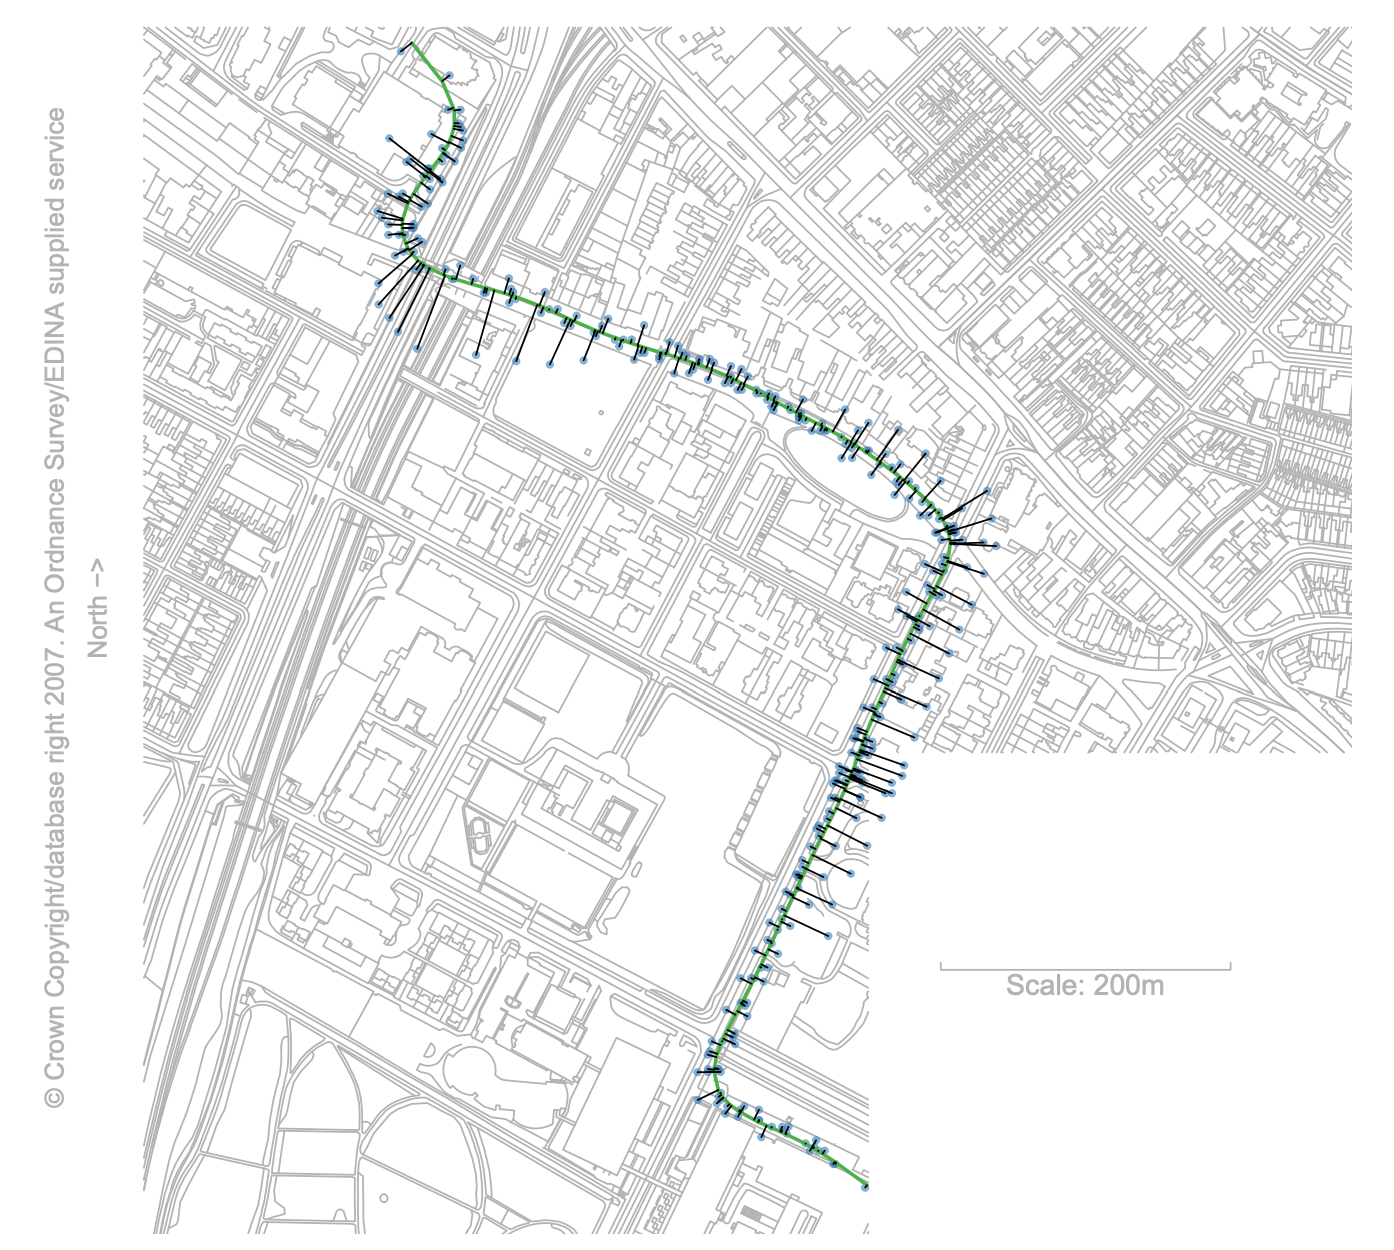
\includegraphics[width=0.9\textwidth]{images/article-map.png}
    \caption{Robust principal curve (green) fitted to GPS point cloud data. Image by Chris Brunsdon, "Path Estimation from GPS Tracks"}
    \label{fig:chrismap}
\end{figure}

Last but not least, authors face a problem with displaying results. Algorithms often return discrete data (points) with various accuracy. It is important to somehow approximate walked path on the map. This task can be achieved using principal curves created from locations grouped into a singular path. Chris Brunsdon in his work\cite{cb} gives a good example of the algorithm for computing such a curve \ref{fig:chrismap}. Einbeck, Tutz and Evers in their work\cite{ete} dive deep into the process of constructing these curves and the benefits from choosing various methods.
